% DCC831 TP1 abstract, written with the official ISMIR 2026 template (ismir.sty is not modified).
\documentclass{article}
\usepackage[T1]{fontenc}
\usepackage[utf8]{inputenc}
\usepackage{ismir} % camera-ready layout: author names, no line numbers
\usepackage{amsmath,cite,url}
\usepackage{graphicx}
\usepackage{booktabs}
\usepackage{color}

% This is a course abstract, not an ISMIR paper: replace the conference header and the
% proceedings line of the copyright notice with the course information.
\makeatletter
\fancyhead[l]{DCC831 Generative AI for Music (UFMG, 2026/2), Assignment 1}
\renewcommand{\permission}{%
  \begin{figure}[b]{%
    \footnotesize
    {
\includegraphics[alt={CC-BY License},height=0.45cm]{cc_by.pdf}}
    \vskip -.45cm
    \begin{spacing}{1.1}
      \hskip 1.5cm \copyright \hskip .1cm \authorname.
      Licensed under a Creative Commons Attribution 4.0 International License (CC BY 4.0).
      Course abstract for DCC831 (UFMG, 2026/2), formatted with the ISMIR 2026 template; it
      was not submitted to ISMIR.
    \end{spacing}
    }
  \end{figure}
}
\makeatother

\title{Evolving 8-Bit Arrangements: A Genetic Algorithm for the NES Four-Voice Idiom}

\oneauthor
  {Giovanni Martinelli}
  {Departamento de Ci\^encia da Computa\c{c}\~ao, Universidade Federal de Minas Gerais}

\def\authorname{G. Martinelli}

\sloppy

\begin{document}

\maketitle

\begin{abstract}
An 8-bit cover is a re-composition: the Nintendo Entertainment System (NES) sound chip has only four monophonic tone channels, so chords must become arpeggios, and a bass line and a drum part must be invented. We present a genetic algorithm (GA) that arranges a lead sheet (melody, chord symbols
and part labels) for the four NES channels. The genotype holds four integer genes per bar, which
select the harmony texture of the second pulse channel, the bass texture of the triangle channel,
the drum pattern of the noise channel and the octave of the melody. Deterministic realizers turn
every genotype into a valid arrangement, so the chip rules hold by construction, and a weighted
mean of seven music-theory criteria scores each genotype. Selection is roulette with windowing and elitism, crossover cuts between bars, and mutation changes each gene with probability 0.01. We arrange two
traditional tunes with famous 8-bit versions, \emph{Ievan Polkka} and \emph{Korobeiniki} (the
Tetris theme), and six Brazilian songs reduced from multi-track MIDI files, and report the
evolution of the fitness, the diversity across seeds, a random-search baseline and a weight
ablation.
\end{abstract}

\section{Introduction}\label{sec:introduction}

Fans re-create songs as 8-bit music, the sound of 1980s consoles. The NES audio processing
unit offers two pulse channels (P1, P2), a triangle channel (TR) and a noise channel (NO), each playing one note at a time, plus a sample channel that we do not use \cite{donahue2018nes}. Within these limits, chiptune composers settled
on a few conventions: fast arpeggios that stand for chords, a dedicated bass voice and
noise-based percussion \cite{driscoll2009endless}. These were aesthetic choices as much as
technical necessities \cite{collins2007loop}. Arranging a song for the chip is therefore a
composition task: the melody is given, but the harmony texture, the bass line, the drum part and
the register must be decided bar by bar.

We use the NES four-voice idiom as the stylistic constraint of a classic algorithmic composition
method, the genetic algorithm. The system receives a lead sheet, written in ABC notation or reduced from a multi-track MIDI file, and outputs a four-track MIDI file that obeys the chip rules, rendered to audio only for listening. To our
knowledge, no earlier GA arranges music for the NES chip; our contribution is to cast the idiom as a searchable space of per-bar textures, while the GA itself is standard. Code, MIDI files, audio (General MIDI and chip renderings), piano rolls and videos of the ten arrangements of eight songs are available at \url{https://github.com/GiowGiow/chiptune-ga-arranger} (folder \texttt{samples/}, one subfolder per piece).

\section{Related Work}\label{sec:related}

Genetic algorithms have arranged existing music for an instrument with physical limits, as in the
guitar arranger of Tuohy and Potter \cite{tuohy2006gabased}; we also treat arranging as search, but
generate new accompaniment for the four NES channels from the chord symbols instead of selecting
notes from a full score. Evolutionary orchestration searches Pareto-optimal combinations of instrument samples that imitate a target sound, under instrumentation constraints \cite{carpentier2010solving}; we address a symbolic counterpart of
this problem with a single weighted fitness. In melody harmonization, Freitas and
Guimar\~aes evolve one chord per bar with a crossover that cuts only at bar boundaries
\cite{freitas2011melody}, and Phon-Amnuaisuk et al.\ report that the rule weights, more than the
operator rates, decide the quality of evolved four-part harmonies \cite{phonamnuaisuk1999evolving};
we adopt the bar-aligned crossover and report a weight ablation. GenJam organizes its genotype in
bars and four-bar phrases \cite{biles1994genjam}, and AMUSE combines normalized music-theory
objectives in a weighted sum \cite{ozcan2008genetic}; our fitness follows the same scheme, with
criteria about the interplay between channels. Evolutionary work on 8-bit music has evolved bytebeat sound formulas with genetic programming and human ratings \cite{kaliakatsos2012interactive}, and LakhNES maps the parts of arbitrary MIDI files onto the NES voices at random to pre-train a Transformer \cite{donahue2019lakhnes}; instead, we search the per-bar textures with explicit musical criteria.

\section{Method}\label{sec:method}

\subsection{Representation}

The lead sheet is parsed into 4/4 bars. Each bar holds its melody notes (MIDI pitch, onset and
duration in beats), its chord segments (root and chord tones), a part label (A, B, \ldots) that
the configuration maps to a role (verse or chorus) and a phrase index (phrases of four bars from
the start of each part, as in GenJam \cite{biles1994genjam}). The genotype (the arrangement plan)
is an integer array with one row per bar and four genes per row; each gene is an index into its
value list in Table~\ref{tab:genes}, so a bar has $5 \times 4 \times 5 \times 3 = 300$ choices and
a 24-bar tune $300^{24}$ genotypes. For each gene value, a deterministic \emph{realizer} writes
the notes of the bar from the chord in effect at each onset: P2 roots sit in C3--B3, TR roots in
E1--D$\sharp$2, drum hits fall on a sixteenth-note grid, and a note outside a channel's range is
folded by octaves into it. Every genotype is thus a valid arrangement, and a validator checks the
chip rules before export: one note at a time per channel, pulse pitches in MIDI 33--108 (a
one-semitone safety margin inside the chip's 32--108 \cite{donahue2018nes}), triangle pitches in
21--108, P2 and TR chord tones on beats 1 and 3 (except the echo, which replays the melody), and
complete bars.

\begin{table}[t]
 \centering
 \footnotesize
 \setlength{\tabcolsep}{3pt}
 \begin{tabular}{@{}llp{0.66\columnwidth}@{}}
  \toprule
  Gene & Channel & Values (indices 0, 1, \ldots) \\
  \midrule
  P2 & pulse 2 & \textbf{hold}: chord root, held; \textbf{arp16}, \textbf{arp32}: chord tones
  cycled up from the root in 16ths or 32nds; \textbf{echo}: the melody an eighth later, softer;
  \textbf{third}: the highest chord tone at least a minor third under each melody note \\
  TR & triangle & \textbf{root}: held root; \textbf{octave pump}: root and octave above
  alternating in eighths; \textbf{root--fifth}: quarters root, fifth, root, fifth;
  \textbf{walking}: quarters root, third, fifth, semitone below the next root \\
  NO & noise & \textbf{none}; \textbf{half time}: kick 1, snare 3, hi-hat 2 and 4;
  \textbf{8th beat}: kick 1 and 3, snare 2 and 4, hi-hat off-beats; \textbf{16th beat}: 8th beat
  plus hi-hat on every sixteenth; \textbf{fill}: 8th beat, then four snare sixteenths; one hit
  per step (kick over snare over hi-hat) \\
  OCT & pulse 1 & \textbf{0}, \textbf{+12}, \textbf{$-$12} semitones \\
  \bottomrule
 \end{tabular}
 \caption{The four genes of each bar and their values. P1 always plays the melody; the GA chooses
 only its octave.}
 \label{tab:genes}
\end{table}

\subsection{Fitness}

The fitness is $f = \sum_i w_i s_i / \sum_i w_i$, the weighted mean of seven criteria
$s_i \in [0, 1]$ with weights $w_i$, as in AMUSE \cite{ozcan2008genetic}; a criterion that does
not apply to a tune (contrast without a chorus) is left out of both sums. With $a_c(b)$ the activity of channel $c$ in bar $b$ (onsets divided by the
16 sixteenth steps, capped at 1, a note density as in \cite{towsey2001towards}):
\emph{complementarity} is the mean of $1 - |a_{\mathrm{P2}}(b) - (1 - a_{\mathrm{P1}}(b))|$, so P2
is calm under a busy melody and busy under a sparse one; \emph{register} is the share of the
sixteenth steps where both P1 and P2 sound in which P2 is lower (1 if they never overlap), a voice-crossing penalty as in GA
harmonization \cite{phonamnuaisuk1999evolving}; \emph{coherence} is the share of adjacent bars inside
a phrase with the same P2, TR, octave and drum genes (a fill may follow any pattern in the bar that
ends the phrase), a repetition objective like the pattern matching of AMUSE \cite{ozcan2008genetic};
\emph{contrast} is $0.5 + \bar{d}_{\mathrm{chorus}} - \bar{d}_{\mathrm{verse}}$ clipped to $[0, 1]$,
with $d$ the mean activity of P2, TR and NO; \emph{bass smoothness} is the mean score of every leap
of the bass line, inside and across bars, 1 up to a fourth, 0 from an octave and linear in between (the upper notes of
the octave pump are an ornament, not leaps), a graded form of the leap rules of
\cite{phonamnuaisuk1999evolving,ozcan2008genetic}; \emph{idiom} is the share of good decisions:
arpeggios on single-chord bars, a chiptune convention \cite{driscoll2009endless}, and drum fills
exactly at phrase ends; \emph{fidelity} is the share of bars where the melody stays in its written
octave, which prevents the degenerate genotype that raises the whole melody to win the register
criterion. The leap thresholds and the default weights (1, with 0.5 for fidelity) are our choices.
Since every realization depends only on its bar and its gene, the system precomputes per-bar score
tables and evaluates a whole population with array indexing.

\subsection{Genetic Operators}

Table~\ref{tab:hyper} lists the hyperparameters. The initial population has 60 random genotypes,
every gene uniform over its values. Parents are drawn by roulette selection with
windowing (probability proportional to the fitness minus the lowest fitness of the generation),
which keeps the selection pressure when the weighted mean gives close values; the two best
genotypes pass unchanged (elitism). One-point crossover, applied to every pair of parents, cuts
only between bars \cite{freitas2011melody}, and mutation replaces each gene by another valid value
with probability 0.01, close to the usual rate $1/L$ \cite{ozcan2008genetic,scirea2017affective}
for the $L = 96$ and 128 genes of the folk tunes. The GA stops after 3000 generations or after 300
generations without improvement (4000 and 400 for the longer MIDI songs). All randomness comes
from one seeded generator, and each run stores its seed, hyperparameters, input hash and code
commit.

\begin{table}[t]
 \centering
 \footnotesize
 \begin{tabular}{@{}ll@{}}
  \toprule
  Hyperparameter & Default (MIDI songs) \\
  \midrule
  Population size; elite count & 60; 2 \\
  Crossover & one point, between bars, rate 1 \\
  Mutation rate, per gene & 0.01 \\
  Max generations; stagnation window & 3000; 300 (4000; 400) \\
  Phrase length & 4 bars \\
  Criterion weights & 1, fidelity 0.5 \\
  \bottomrule
 \end{tabular}
 \caption{GA hyperparameters. Every run uses these values unless stated otherwise.}
 \label{tab:hyper}
\end{table}

\subsection{Inputs and Rendering}

ABC lead sheets give the melody, the chords and the part labels directly. A multi-track MIDI song
is first reduced to a lead sheet. The chosen melody track or tracks are merged by a skyline (the
highest note wins) and snapped to a sixteenth-note grid. One chord per half bar is chosen among
major, minor, dominant-seventh and minor-seventh chords: the other tracks vote for pitch classes in
proportion to how long they sound, bass tracks count twice, and a chord whose root is the bass note
gets a bonus. The arrangement is rendered twice from the same MIDI file: with General MIDI
timbres (FluidSynth) and with our own NES chip synthesizer (pulse, triangle and noise waveforms).

\section{Results}\label{sec:results}

\textbf{Setup.} We arranged two traditional tunes with well-known 8-bit versions: \emph{Ievan
Polkka}, with the melody as sung by Loituma, in E-flat minor at 110 BPM, with form A B A$'$ played
twice (24 bars), and \emph{Korobeiniki}, the Tetris theme, in A minor at 150 BPM, with form A A B A
(32 bars). The B parts are labeled chorus.
All runs on these two tunes stopped by stagnation, after 717 to 1986 generations.

\textbf{Evolution.} Figure~\ref{fig:evolution} shows a typical run. The best fitness rises from
0.58 in the random generation 0 to 0.92, and the mean fitness follows it closely. The share of distinct genotypes stays above 0.86: the genotypes become similar, but mutation keeps most of them
different. Between generation 0 and the final genotype, the coherence of Korobeiniki goes
from 0 to 0.92 and its fidelity from 0.41 to 1.

\begin{figure}[t]
 \centerline{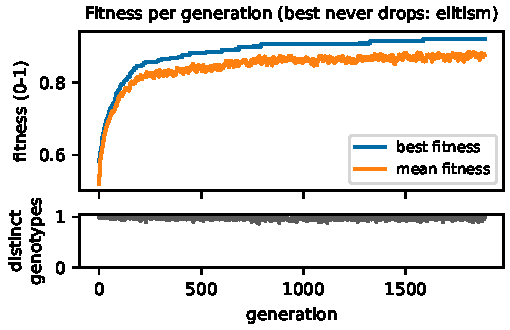
\includegraphics[width=\columnwidth]{figures/korobeiniki-s1-evolution.pdf}}
 \caption{Korobeiniki, seed 1. Top: best and mean fitness per generation. Elitism keeps the best curve non-decreasing. Bottom: share of distinct genotypes in the population.}
 \label{fig:evolution}
\end{figure}

\textbf{Search against chance.} Table~\ref{tab:experiments} compares five seeds with a random
search that scores as many random genotypes as the first GA run did (43,080 and 113,220 for the
two folk tunes). Random search stays near 0.6 because it never finds coherent phrases (coherence
near 0), while every GA run on the folk tunes reaches 0.88 to 0.94. The seeds end on different
genotypes: on average, 28\% (Ievan Polkka) and 32\%
(Korobeiniki) of the genes differ between two seeds. The same configuration therefore yields
different arrangements, as the assignment requires.

\begin{table}[t]
 \centering
 \footnotesize
 \setlength{\tabcolsep}{4pt}
 \begin{tabular}{@{}lccc@{}}
  \toprule
  & Ievan Polkka & Korobeiniki & 6 MIDI songs \\
  \midrule
  GA, mean of 5 seeds & 0.92 & 0.90 & 0.87 \\
  GA, worst seed & 0.91 & 0.88 & 0.82 \\
  Random search & 0.64 & 0.62 & 0.60 \\
  Genes differing & 28\% & 32\% & 36\% \\
  \midrule
  \multicolumn{4}{@{}l}{\emph{Ablation, seed 1: criterion score, default weight $\rightarrow$ 0}} \\
  coherence & 0.83 $\rightarrow$ 0.28 & 0.92 $\rightarrow$ 0.63 & 0.84 $\rightarrow$ 0.31 \\
  contrast & 1.00 $\rightarrow$ 0.55 & 0.93 $\rightarrow$ 0.39 & 0.90 $\rightarrow$ 0.54 \\
  bass smoothness & 1.00 $\rightarrow$ 0.78 & 0.97 $\rightarrow$ 0.90 & 0.93 $\rightarrow$ 0.87 \\
  idiom & 1.00 $\rightarrow$ 0.86 & 0.94 $\rightarrow$ 0.69 & 0.92 $\rightarrow$ 0.66 \\
  fidelity & 0.92 $\rightarrow$ 0.50 & 1.00 $\rightarrow$ 0.44 & 0.92 $\rightarrow$ 0.27 \\
  register & 1.00 $\rightarrow$ 0.94 & 1.00 $\rightarrow$ 0.96 & 0.94 $\rightarrow$ 0.86 \\
  complementarity & 0.64 $\rightarrow$ 0.56 & 0.73 $\rightarrow$ 0.71 & 0.72 $\rightarrow$ 0.61 \\
  \bottomrule
 \end{tabular}
 \caption{Fitness with the default weights. Random search scores as many genotypes as the first
 GA run; genes differing: mean share of genes that differ between two seeds. The MIDI column averages
 the six songs. Ablation: removing a criterion lowers its own score in every case.}
 \label{tab:experiments}
\end{table}

\textbf{Ablation and hyperparameter variation.} Setting one weight to 0 lowers that criterion
(Table~\ref{tab:experiments}). Without fidelity, the GA moves about half of the bars of the melody
by an octave; without coherence, it changes textures inside phrases; without contrast, the chorus
loses its denser accompaniment. Register and complementarity move least: most P2 textures sit
below the melody, and the texture vocabulary limits how closely P2 can mirror the activity of the
melody. The submitted pieces vary the seed (samples korobeiniki-s1 and korobeiniki-s2) and the
fidelity weight (ievan-polkka-s1 and ievan-polkka-s1-fidelity0). With fidelity at 0, the GA
raises 12 of the 24 melody bars by an octave, so the melody jumps between registers, and the A
parts move to held chords over the octave pump.

\textbf{Listening.} In Ievan Polkka (seed 1), the A parts hold a chord tone under the melody over a
root bass and light drums, the B parts switch to fast arpeggios over the octave pump, a typical NES
bass, with a sixteenth-note beat, and a fill closes every phrase. Korobeiniki arpeggiates
throughout, with a root bass and fills only in the A parts, and plays the octave pump and a
sixteenth-note beat in the bridge (B). The noise channel sounds 36\% to 48\% of the time, close to
the 39\% measured in NES game music, but our P2 and TR channels almost never rest (99--100\%,
against 84\% and 70\% in that corpus \cite{donahue2018nes}).

\textbf{MIDI songs.} We also arranged excerpts (32--56 bars) of six Brazilian songs from fan-made
MIDI files: \emph{Voa Voa}, \emph{Mulher de Fases}, \emph{Amor I Love You}, \emph{Por Voc\^e},
\emph{Aquarela} and \emph{Fico Assim Sem Voc\^e}.
In four files, the embedded lyric syllables identify the sung melody track; in the other two, the
melody is the monophonic line that plays throughout. These runs use the MIDI settings of
Table~\ref{tab:hyper} and stopped after 1182 to 4000 generations (4 of the 30 seed runs reached
the cap). We repeated the experiments on every song (last column of Table~\ref{tab:experiments}).
The GA beats random search on each song (five-seed means 0.84--0.89 against 0.57--0.62), the seeds
differ more (36\% of the genes), and removing a criterion lowers its own score on every song. The
songs score lower than the folk tunes on average (0.87 against 0.91). Their melodies often sit in
octaves 3--4, so keeping the written register conflicts with keeping P2 below the melody (seed 1:
fidelity 0.75--1.00, register 0.87--1.00), and coherence is lower (0.69--0.92, against 0.83 and
0.92 for the folk tunes at seed 1).

\section{Discussion and Future Work}\label{sec:discussion}

The search, not chance, produces the arrangements, but the approach has clear limits. The fitness is a weighted mean of hand-written heuristics, a common choice whose weights are hard to tune \cite{fernandez2013ai} and that hides the conflicts between objectives. A Pareto front \cite{freitas2011melody,carpentier2010solving}
would expose these trade-offs. Automatic chord detection on MIDI songs is approximate, and we did not measure its errors. The textures come from a fixed vocabulary, so the GA chooses between arranging gestures but does
not invent new ones; the bass never rests, and only 4/4 is supported. Our chip synthesizer has one
fixed duty cycle per pulse channel and no envelopes or pitch effects. Future work: a fitness learned from the NES Music
Database \cite{donahue2018nes}, evolved variations of the P2 and TR lines, and an A/B listening
test as in \cite{donahue2019lakhnes}.

\bibliography{references}

\end{document}
